%% modified for 336VD at FEL CVUT
%% bare_jrnl.tex
%% V1.2
%% 2002/11/18
%% by Michael Shell
%% mshell@ece.gatech.edu
\documentclass[journal]{IEEEtran}
%\usepackage{czech}
\usepackage{graphicx}

\begin{document}
%
% paper title
\title{Kmeans pro Poker Hands}
\author{Martin Luke\v{s}
}

\markboth{SEMESTRAL WORK, COURSE 336VD: DATA MINING, CZECH TECHNICAL UNIVERSITY IN PRAGUE, 2009/10}{Shell \MakeLowercase{\textit{et al.}}: Bare Demo of IEEEtran.cls for Journals}
\maketitle


\begin{abstrakt}
Rozpozn\'an\'i s\'ily ruky v pokeru spolu s pozorov\'an\'im tell\r{u} (man\'yr, v\'yraz, emoce \v{c}i zvyk vyjad\v{r}uj\'{i}c\'{i} informaci o stavu ruky hr\'{a}\v{c}e) odd\v{e}luj\'i \v{s}patn\'{e} hr\'a\v{c}e od dobr\'ych. Tento dokument se zam\v{e}ril na zkoum\'{a}n\'{i} s\'{i}ly jednotliv\v{y}ch rukou.
\end{abstrakt}

\section{Assignment}
Vyberte si data, kter\'{a} jsou pou\v{z}iteln\'{a} pro klasifikaci nebo
regresi. Data p\v{r}edzpracujte a naimportujte do DM aplikace.
Zvolte si shlukovac\'{i} algoritmus (k-means, hierarchick\'{e} shlukov\'{a}n\'{i},
SOM). Najd\v{e}te nastaven\'{i} parametr\r{u} zvolen\'{e}ho algoritmu tak,
aby produkoval co nejlep\v{s}\'{i} v\'{y}sledky. Interpretujte v\'{y}sledky.

\section{Introduction}
 Jako shlukovac\'{i} algoritmus jsem si vybral K-means. Data byla ji\v{z} v \v{c}\'{i}seln\'{e} podob\v{e} a bylo nutn\'{e} je jen normalizovat.
Atributy a jejich v\'{y}znam je zachycen v tabulce 1. Posledn\'{i} atribut Hand Power je tzv. u\v{c}itel, kter\'{y} vyjad\v{r}uje s\'{i}lu dan\'{e} ruky. Polo\v{z}ek v datech je p\v{r}es jeden milion, proto jsem pou\v{z}il n\'{a}hodn\'{y} vzorek asi 3000 instanc\'{i}, kter\'{y} pro m\'{e} \'{u}\v{c}ely posta\v{c}il.
%


\begin{table}
%% increase table row spacing, adjust to taste
\renewcommand{\arraystretch}{1.3}
\caption{Taulka atribut\r{u}}
\label{table_example}
\centering
%% Some packages, such as MDW tools, offer better commands for making tables
%% than the plain LaTeX2e tabular which is used here.
\begin{tabular}{|c|c|c|}

\hline
Atribut & V\'{y}znam & Rozsah \\
\hline
\hline
C1 & Barva prvn\'{i} karty & 1-4\\
\hline
S1 & Hodnota prvn\'{i} karty & 1-13\\
\hline
C2 & Barva druh\'{e} karty & 1-4\\
\hline
S2 & Hodnota druh\'{e} karty & 1-13\\
\hline
C3 & Barva t\v{r}et\'{i} karty & 1-4\\
\hline
S3 & Hodnota t\v{r}et\'{i} karty & 1-13\\
\hline
C4 & Barva \v{c}tvrt\'{e} karty & 1-4\\
\hline
S4 & Hodnota \v{c}tvrt\'{e} karty & 1-13\\
\hline
C5 & Barva p\'{a}t\'{e} karty & 1-4\\
\hline
S5 & Hodnota p\'{a}t\'{e} karty & 1-13\\
\hline
Hand Power & S\'{i}la ruky & 0-11\\
\hline



\end{tabular}
\end{table}
\section{Methodology}
K-means je shlukovac\'{i} algoritmus, kter\'{y} je za\v{r}azov\'{a}n do skupiny tzv centroidn\'{i}ch algoritm\r{u}. K-means nahrazuje v\v{s}echny shluky jejich reprezentanty (centroidy) a nemus\'{i} tak vypo\v{c}\'{i}t\'{a}vat v\v{s}echny vzd\'{a}lenosti, ale jen vzd\'{a}lenosti v\v{s}ech bod\r{u} od centroid\r{u}.


K m\v{e}\v{r}en\'{i} vzd\'{a}lenost\'{i} m\r{u}\v{z}eme vyu\v{z}\'{i}t r\r{u}zn\'{y}ch m\v{e}\v{r}\'{i}c\'{i}ch metod (metrik). V pokusech byla pou\v{z}ita eukleidovsk\'{a}, manhattansk\'{a} a cosinova metrika. Eukleidovsk\'{a} - E(P,Q) - metrika m\v{e}\v{r}\'{i} vzd\'{a}lenost dvou bod\r{u} (P a Q) v n-rozm\v{e}rn\'{e}m prostoru jako odmocninu z sou\v{c}tu kvadr\'{a}t\r{u} rozd\'{i}l\r{u} odpov\'{i}daj\'{i}c\'{i}ch sou\v{r}adnic.



\begin{eqnarray*}
P&=&(p_1,p_2,\ldots,p_n)\\
Q&=&(q_1,q_2,\ldots,q_n)\\
E(P,Q)&= &\sqrt{\sum_{k=1}^{n}{(p_k-q_k)^2}}
\end{eqnarray*}

Manhattansk\'{a} metrika - M (P,Q) - m\v{e}\v{r}\'{i} vzd\'{a}lenost dvou bod\r{u} (P a Q) v n-rozm\v{e}rn\'{e}m prostoru jako sou\v{c}et absolutn\'{i}ch hodnot rozd\'{i}l\r{u} odpov\'{i}daj\'{i}c\'{i}ch sou\v{r}adnic.

\begin{eqnarray*}
P&=&(p_1,p_2,\ldots,p_n)\\
Q&=&(q_1,q_2,\ldots,q_n)\\
M(P,Q)&= &\sum_{k=1}^{n}{\left| p_k-q_k \right|}
\end{eqnarray*}

Kosinova metrika - dist (P,Q) - je hodnota podobnosti (\'{u}hlu), kter\'{y} sv\'{i}raj\'{i} P a Q.
\begin{eqnarray*}
P&=&(p_1,p_2,\ldots,p_n)\\
Q&=&(q_1,q_2,\ldots,q_n)\\
dist(P,Q)&= &\arccos{\frac{\sum_{k=1}^{n}{ p_k*q_k }}{\sqrt{\sum_{k=1}^{n}{p_k^2}*\sum_{k=1}^{n}{q_k^2}}}}=\\
&=&\arccos{(\frac{P*Q}{\left|P\right|*\left|Q\right|})}
\end{eqnarray*}

Na Figure 1 vid\'{i}me porovn\'{a}n\'{i} v\v{s}ech t\v{r}\'{i} metrik. Nez\'{a}visl\'{a} prom\v{e}nn\'{a} je po\v{c}et centroid\r{u} a z\'{a}visl\'{a} je hodnota silhouette. Data jsou nejl\'{e}pe shlukovan\'{a} pro dva shluky u v\v{s}ech metrik. Na Figure 2, 3, 4 vid\'{i}me grafy pro nejlep\v{s}\'{i} po\v{c}ty shluk\r{u} (2).


\begin{table}
\renewcommand{\arraystretch}{1.3}
\caption{Tabulka porovn\'{a}vaj\'{i}c\'{i} vzd\'{a}lenosti podle hodnoty silhouette}
\label{table_example}
\centering
\begin{tabular}{|c|c|c|c|c|}

\hline
Po\v{c}et shluk\r{u} & Eukleidovsk\'{a} vzd & Manhattonsk\'{a} vzd & Cosinova vzd \\
\hline
\hline
2 &	0,17 &	0,09 &	0,17\\
\hline
5 &	0,15 &	0,07 &	0,16\\
\hline
10 &	0,15&	0,06&	0,15\\
\hline
15	&0,15&	0,07&	0,16\\
\hline
20&	0,15&	0,07&	0,16\\
\hline
\end{tabular}
\end{table}

\begin{figure}[!h]
\begin{center}
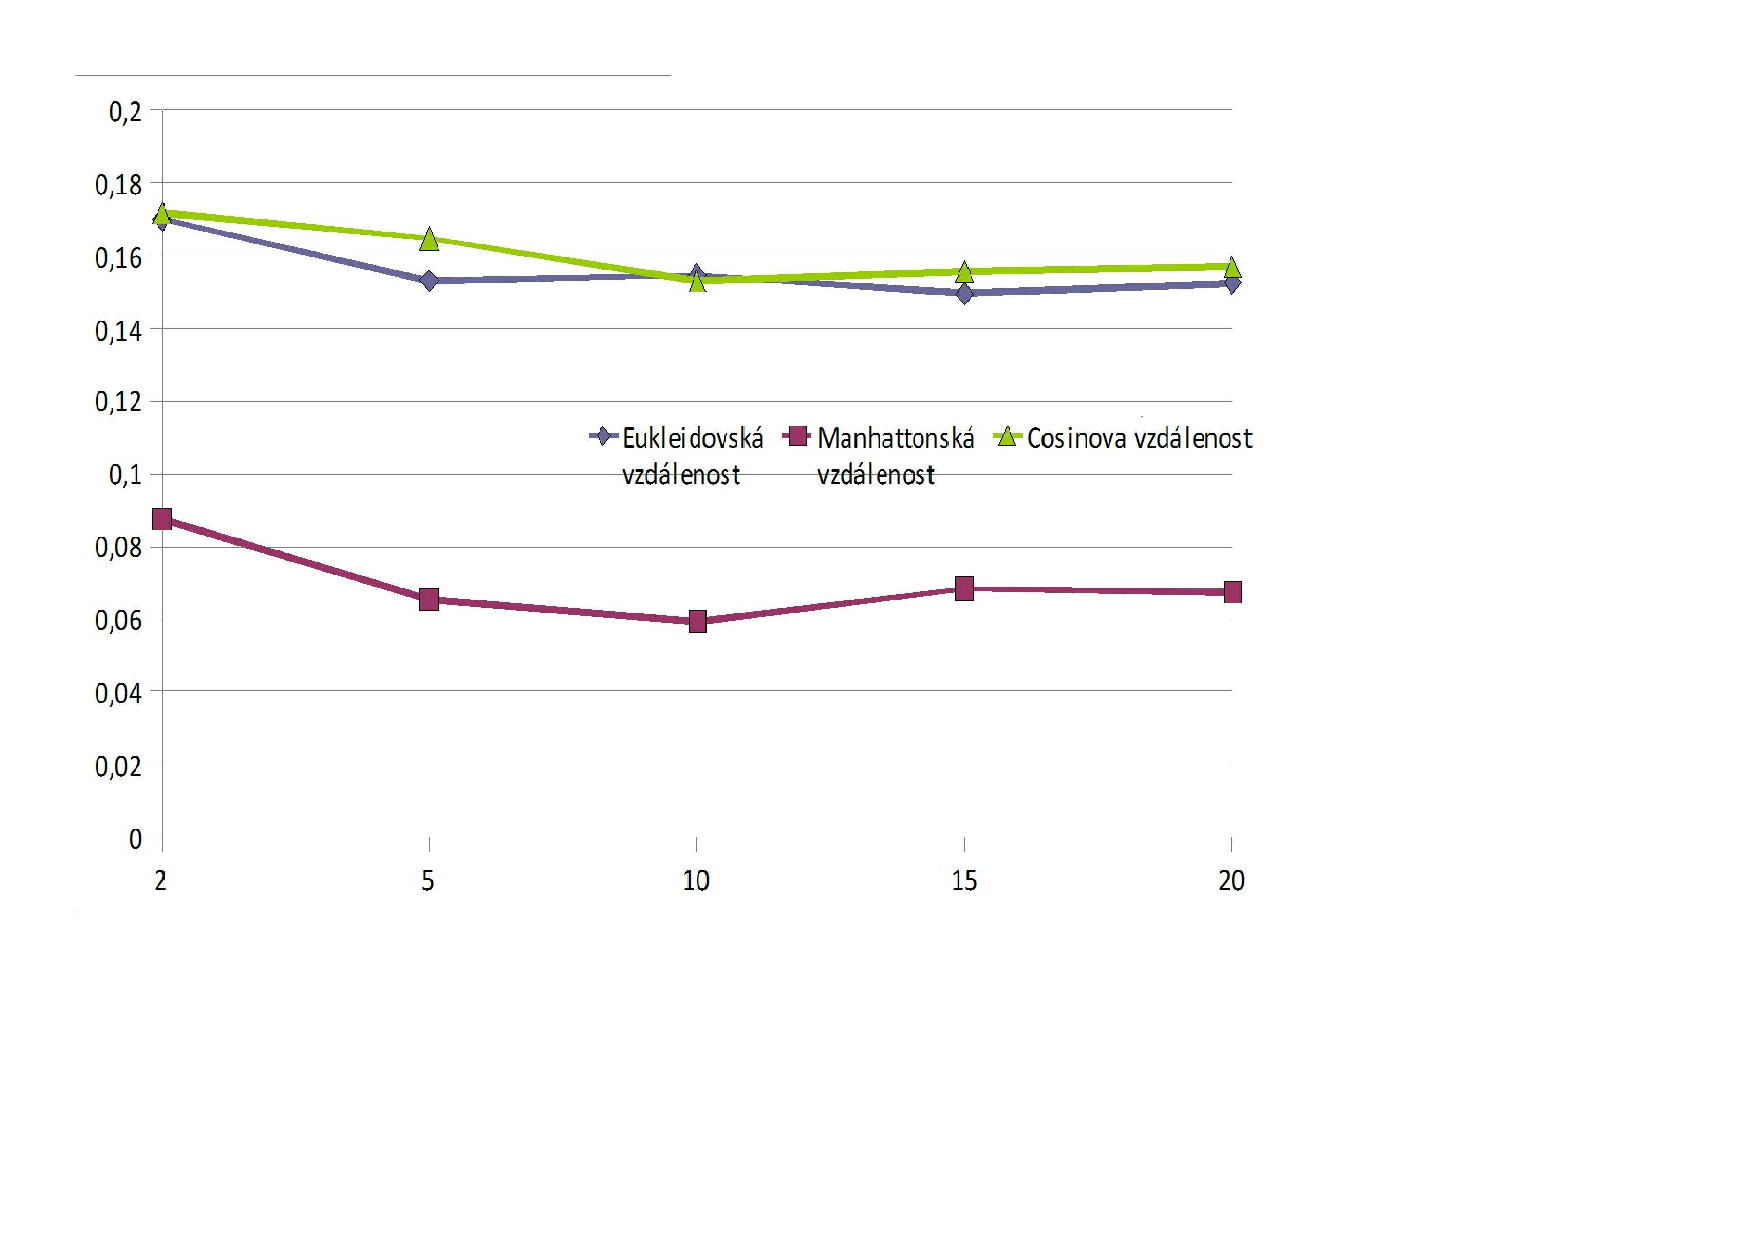
\includegraphics[width=4in]{porovnani_vzd.pdf}
\caption{Graf porovn\'{a}n\'{i} metrik podle hodnoty silhouette}
\end{center}\label{f-ac}
\end{figure}

\begin{figure}[!h]
\begin{center}
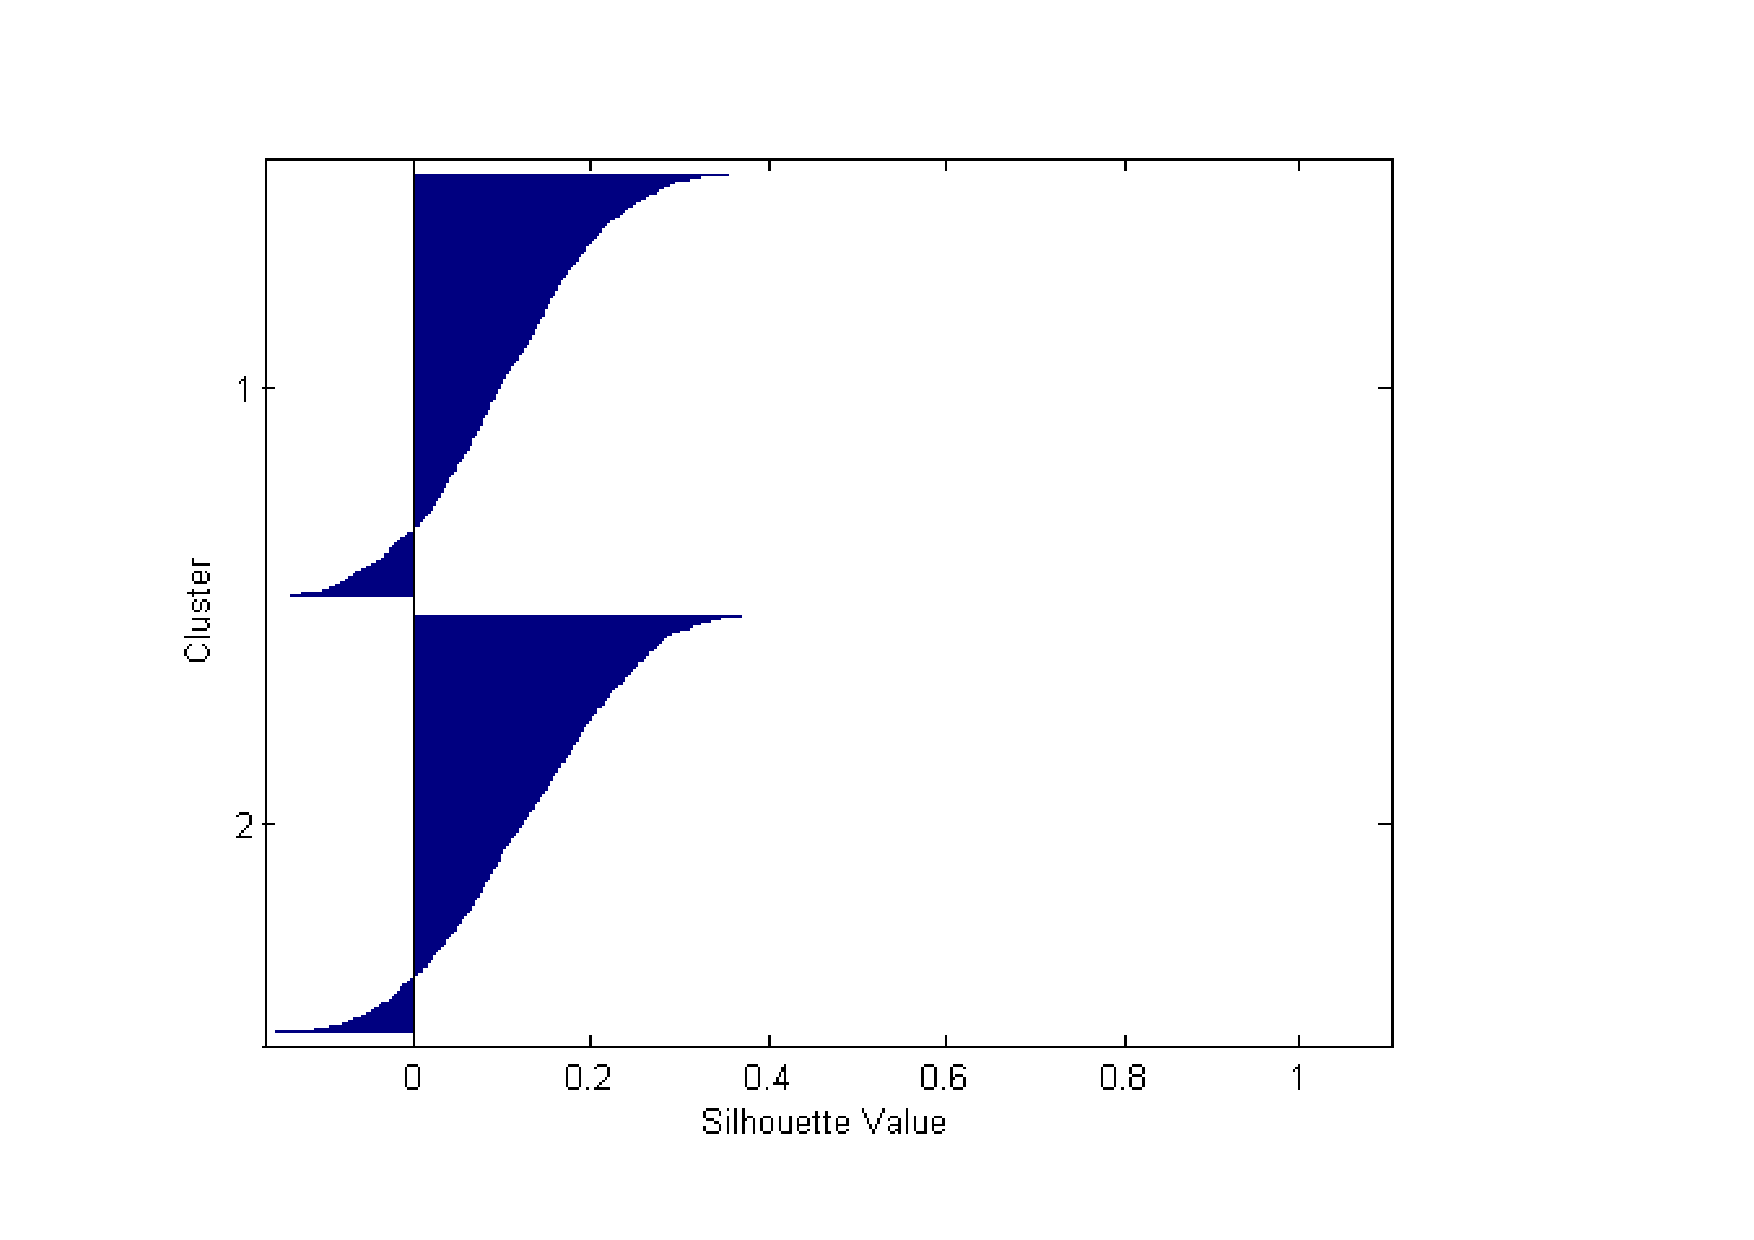
\includegraphics[width=4in]{manhattan.pdf}
\caption{Silueta Manhattansk\'{e} vzd }
\end{center}\label{f-ac}
\end{figure}

\begin{figure}[!h]
\begin{center}
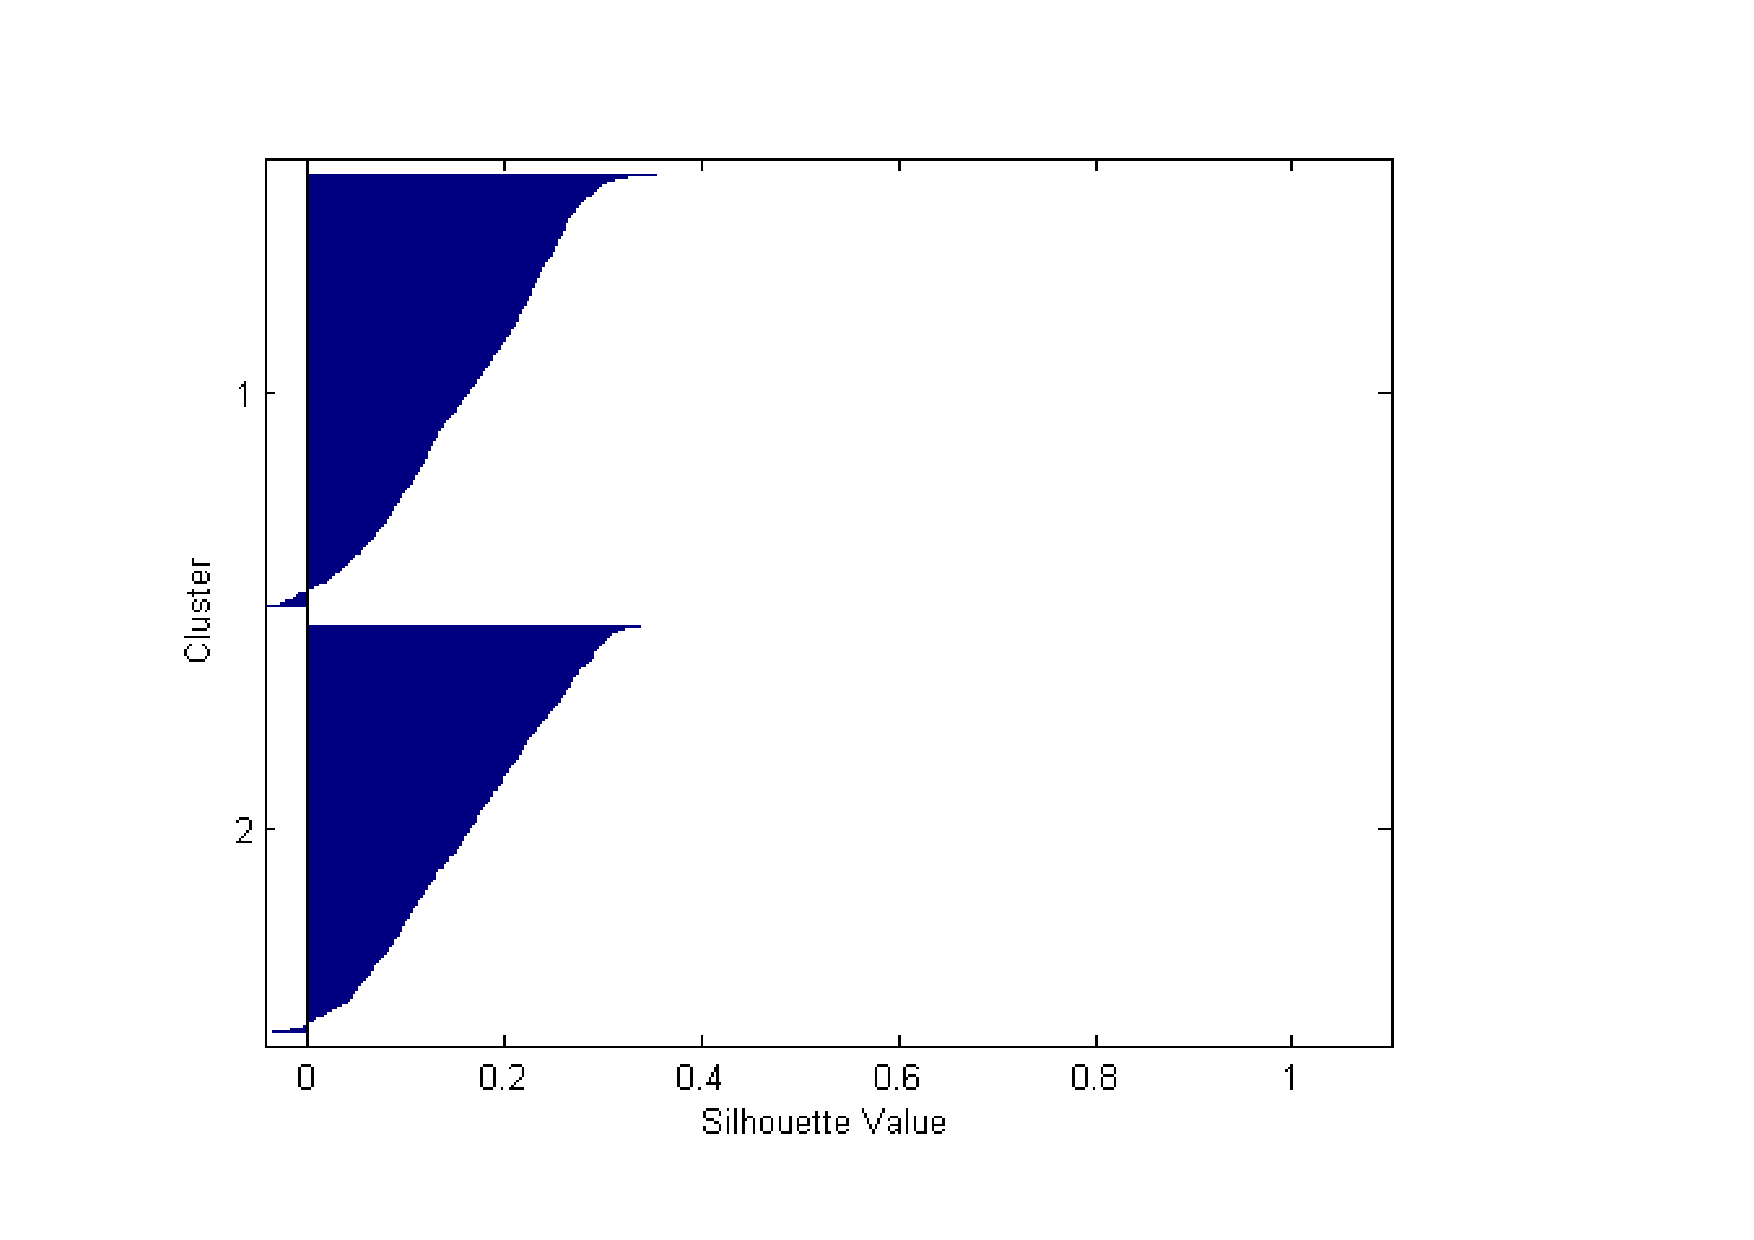
\includegraphics[width=4in]{cos.pdf}
\caption{Silueta Cosinovy vzd }
\end{center}\label{f-ac}
\end{figure}

\begin{figure}[!h]
\begin{center}
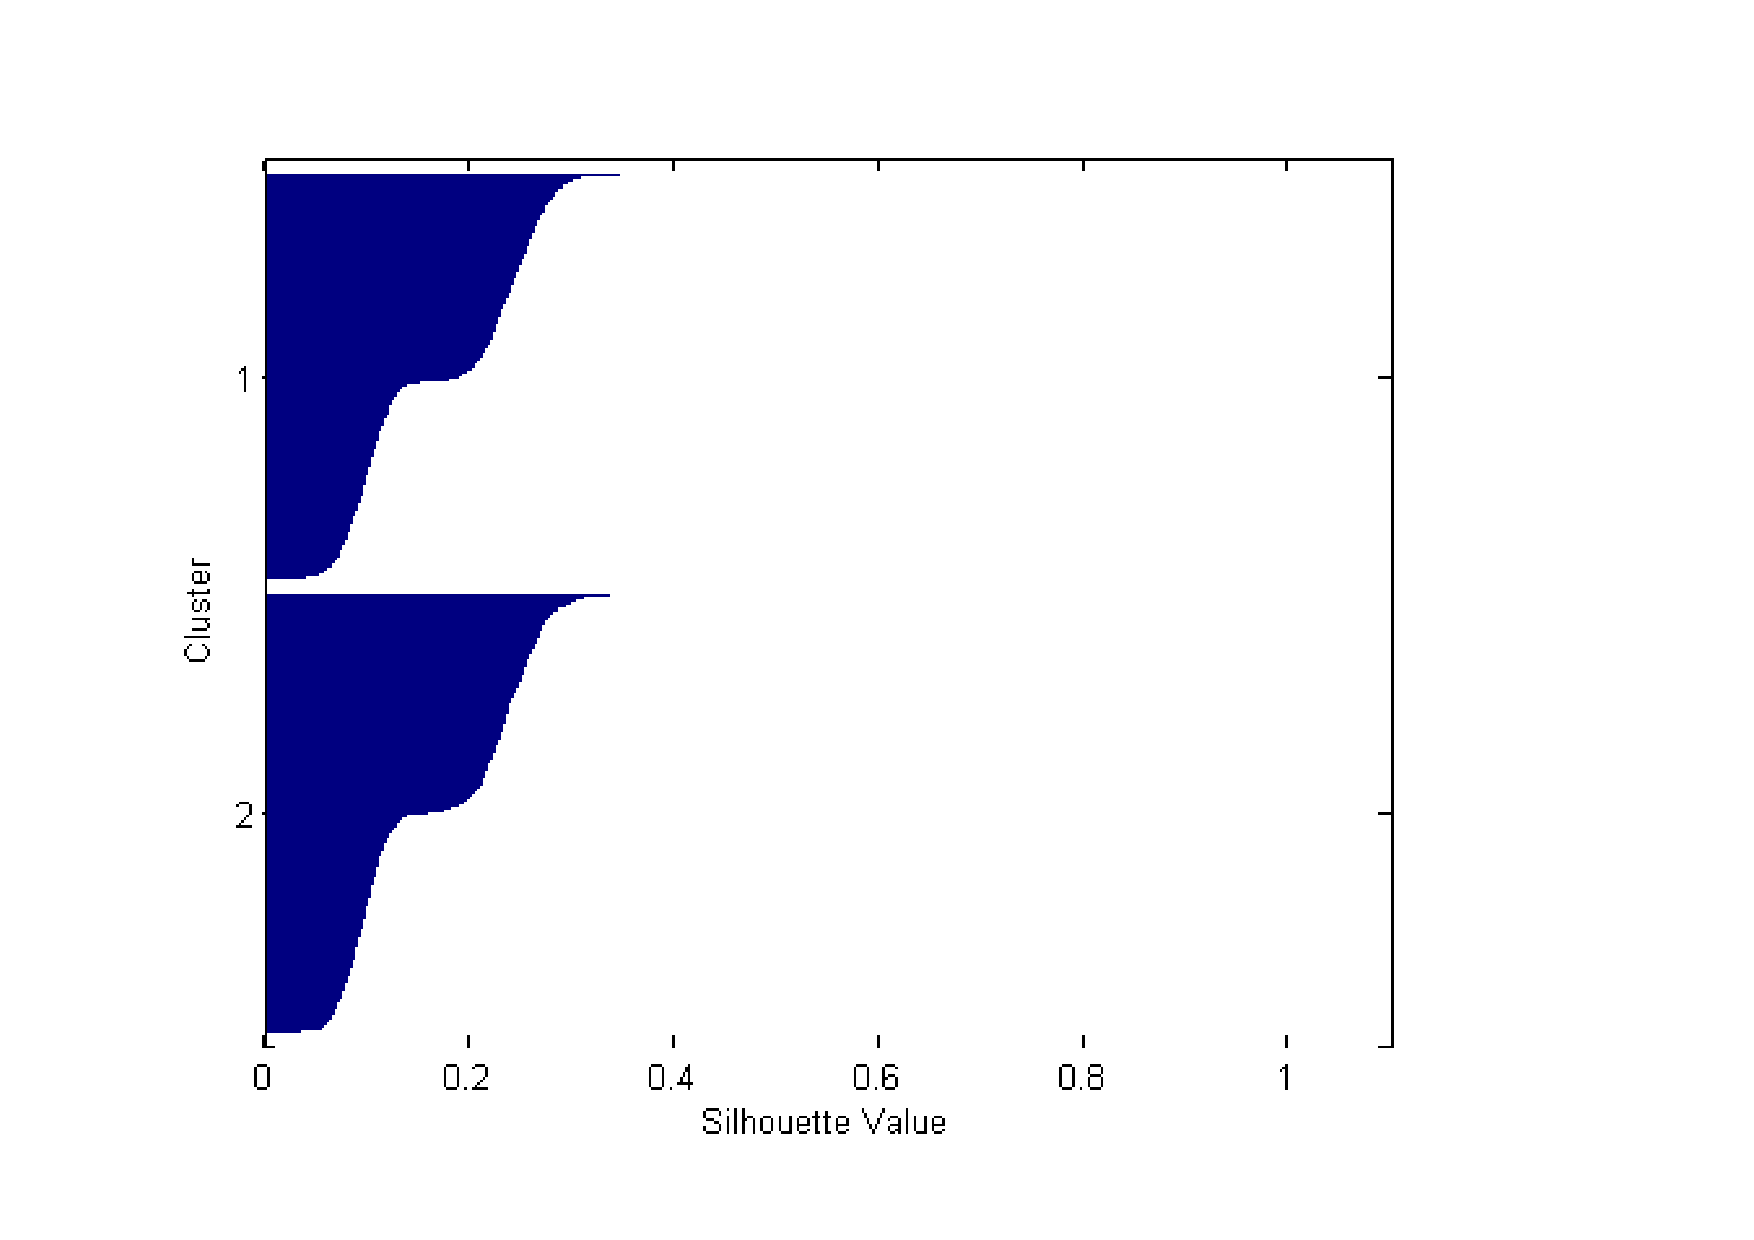
\includegraphics[width=4in]{euklid.pdf}
\caption{Silueta Eukleidovsk\'{e} vzd }
\end{center}\label{f-ac}
\end{figure}


\section{Conclusion}
P\v{r}i m\v{e}\v{r}en\'{i} jsem zjistil, \v{z}e model je nejlep\v{s}\'{i} pro po\v{c}et shluk\r{u} roven 2 u v\v{s}ech metod, co\v{z} je trochu zvl\'{a}\v{s}tn\'{i}. Je mo\v{z}n\'{e}, \v{z}e data nejsou pro K-means \'{u}pln\v{e} ide\'{a}ln\'{i}, proto\v{z}e jeden parametr je nejlep\v{s}\'{i} pro v\v{s}echny modely, nav\'{i}c pro dva s absolutn\v{e} stejnou hodnotou silhouette. Nejl\'{e}pe tedy dopadl model Cosinovy a Eukleidovsk\'{e} vzd\'{a}lenosti.

\begin{literatura}{1}
\bibitem{IEEEhowto:kopka}
Materi\'{a}ly z p\v{r}edn\'{a}\v{s}ek.

\end{literatura}

\end{document}


